\documentclass[pdftex,12pt,a4paper]{report}

\usepackage[portuguese,english]{babel}
\usepackage[T1]{fontenc} 
\usepackage[table,xcdraw]{xcolor}
\usepackage[utf8]{inputenc}
\usepackage[pdftex]{graphicx}
\usepackage{minitoc}
\usepackage{hyperref}
\usepackage{indentfirst}
\usepackage[compact]{titlesec}
\usepackage{fancyhdr}
\usepackage{caption}
\usepackage{pgfplots}
\usepackage{pgfplotstable}
\usepackage{fixltx2e}
\usepackage{mathtools}
\usepackage{fancyhdr}
\usepackage{listings}
\usepackage{color}
\usepackage{sverb}
\usepackage[section]{placeins}
\usepackage{adjustbox}
\titleformat*{\subsubsection}{\itshape}


%Highlight
\newcommand{\shellcmd}[1]{\indent\indent\texttt{\footnotesize\# #1}\\}

\pagestyle{fancy}
\renewcommand*\thesection{\thechapter\arabic{section}}
\newcommand{\HRule}{\rule{\linewidth}{0.5mm}}
\begin{document}

\begin{titlepage}

\begin{center}


\includegraphics[width=0.15\textwidth]{./logo}\\[0.5cm]    

\textsc{\large Universidade de Aveiro \\[1cm]\large departamento de electrónica, telecomunicações e informática}\\[1cm]

\textsc{\large{1}\large - Desempenho e Dimensionamento de Redes\\[1cm]}

\HRule \\[0.5cm]
{ \huge \bfseries abs}\\[0.4cm]
{ \large \bfseries x}\\[0.4cm]
\HRule \\[1cm]

\textsc{\small{8240 - MESTRADO INTEGRADO EM ENGENHARIA DE COMPUTADORES E TELEMÁTICA}}\\[1cm]

\begin{minipage}{0.4\textwidth}

\begin{flushleft} \large
\href{mailto:rafael.ferreira@ua.pt}{António Rafael da \\ Costa Ferreira }
 \small{\\NMec: 67405}
\end{flushleft}
\end{minipage}
\begin{minipage}{0.4\textwidth}

\begin{flushright} \large
\href{mailto:rodrigocunha@ua.pt}{Rodrigo Lopes \\ da Cunha}
\small{\\NMec: 67800}
\end{flushright}
\end{minipage}\\[1cm]

{\large Docente: Paulo Salvador }\\[0.5cm]

\vfill

{\large Fevereiro de 2016 \\ 2015-2016}

\end{center}

\end{titlepage} %Titulo do Relatorio
\renewcommand{\headrulewidth}{0pt}

%Cabeçalhos de rodapé
\fancyhead{}
\fancyfoot{}
\lhead{Network Traffic Engineering}
\rhead{DDR - 2015/2016}
\lfoot{Rafael Ferreira nmec: 67405 \\ Rodrigo Cunha nmec: 67800}
\rfoot{\thepage}

%Renomear Comandos
\renewcommand*\contentsname{Conteúdos}
\renewcommand*\figurename{Figura}
\renewcommand*\tablename{Tabela}

%Conteúdos, dar paragrafo
\tableofcontents
%Headers
\renewcommand{\headrulewidth}{0.15pt}
\renewcommand{\thechapter}{}

\clearpage

\section{Virtual-Circuit Switched Network}

\subsection{Exercício 1}

Para iniciar este trabalho foi-nos dado vários ficheiros de base. O ficheiro NetGen.py é responsável por gerar uma rede, com vários nós que inclui o nome e localização geográfica, e as ligações inter-nó, matrizes de tráfego que define os fluxos de tráfego entre todas as cidades/ nós.

A localização geográfica (pos) é obtida dinamicamente a partir do nome do no (nome da cidade) usando a API do Google Maps, ficheiro getGeo.py. 

A matriz de tráfego (TM) é gerado aleatóriamente. É possível também guardar o resultado num ficheiro .dat e passando como argumento o parâmetro -f, net.dat.

\begin{figure}[!htb]
  \centering
  \begin{minipage}[b]{0.4\textwidth}
    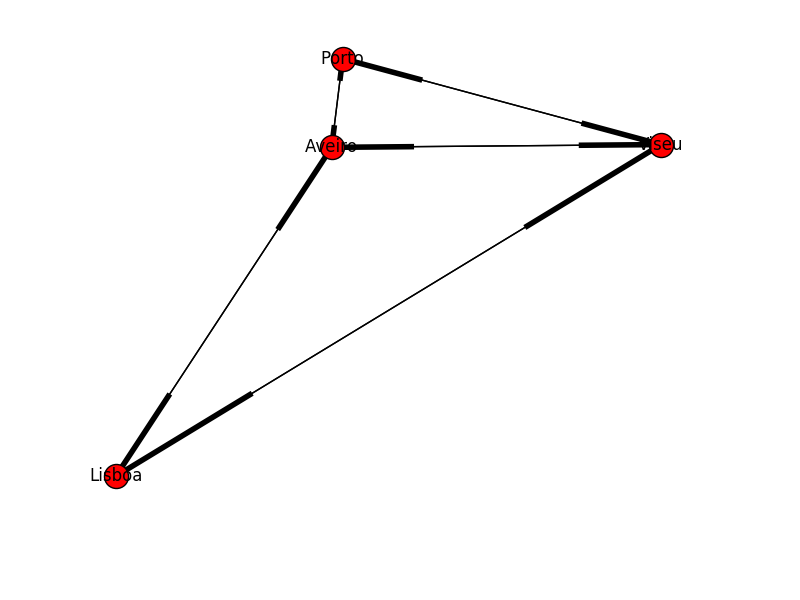
\includegraphics[width=\textwidth]{imagensGuia/esquema_rede_pequena.png}
  \end{minipage}
  \hfill
  \begin{minipage}[b]{0.4\textwidth}
    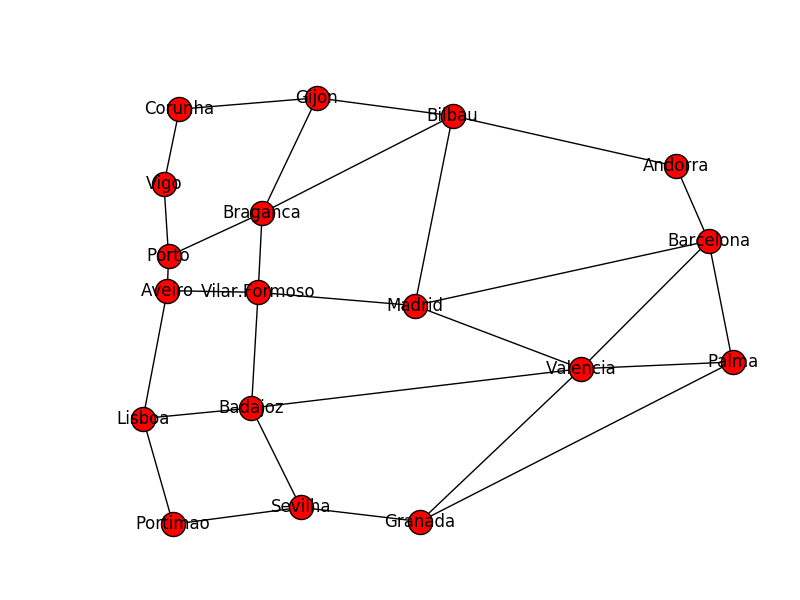
\includegraphics[width=\textwidth]{imagensGuia/esquema_rede_grande.png}
  \end{minipage}
  \caption{Rede pequena de teste e rede grande}
\end{figure}


\subsection{Exercício 2, 3 e 4}

No exercício 2 é usado o caminho mais curto como escolha para o caminho entre pontos, sendo que isto é dado pela soma das conexões e usando o algoritmo Greedy.

No exercício 3, foi calculado o "average one-way delay" e a carga em todas as direções em todos os links.

Para isso, para calcular o "average one-way delay", foi usada a seguinte fórmula baseada na aproximação Kleinrock:

$\mu$ = 1e9 / 8000 , é igual ao link speed em pkts/sec (1Gbps)

\[W = 1e6\times\left[\frac{1}{\left(\mu-atraso\right)}\right]\]

Para calcular o atraso, teve de se criar um ciclo de forma a percorrer todos os links e criar uma lista com os atrasos.

\begin{lstlisting}[language=python]
for pair in allpairs:
    path = sol[pair]
    for i in range(0, len(path) - 1):
        ws_delay[pair] = 1e6 / (mu - \
        net[path[i]][path[i + 1]]['load'])
\end{lstlisting}

Após isso foi possível apresentar a seguinte tabela para a rede pequena:

\begin{table}[!htb]
        \centering
        \resizebox{\textwidth}{!}{\begin{tabular}{|l|l|l|l|l|}
\hline
\multicolumn{1}{|c|}{\textbf{Origem}} & \multicolumn{1}{|c|}{\textbf{Destino}} & \multicolumn{1}{|c|}{\textbf{Saltos}} & \multicolumn{1}{|c|}{\textbf{Carga (pkts/sec)}} & \multicolumn{1}{|c|}{\textbf{Atraso (micro/sec)}} \\ \hline
Lisboa & Viseu & Lisboa, Viseu & 31271 & 10.67 \\ \hline
Porto & Lisboa & Porto, Aveiro, Lisboa & Indisponível & 31.86 \\ \hline
Viseu & Porto & Viseu, Porto & 31401 & 10.68 \\ \hline
Lisboa & Aveiro & Lisboa, Aveiro & 62675 & 16.04 \\ \hline
Aveiro & Viseu & Aveiro, Viseu & 31199 & 10.66 \\ \hline
Viseu & Aveiro & Viseu, Aveiro & 31378 & 10.68 \\ \hline
Aveiro & Porto & Aveiro, Porto & 63050 & 16.14 \\ \hline
Porto & Viseu & Porto, Viseu & 31396 & 10.68 \\ \hline
Porto & Aveiro & Porto, Aveiro & 62129 & 15.91 \\ \hline
Lisboa & Porto & Lisboa, Aveiro, Porto & Indisponível & 32.19 \\ \hline
Viseu & Lisboa & Viseu, Lisboa & 31171 & 10.66 \\ \hline
Aveiro & Lisboa & Aveiro, Lisboa & 62304 & 15.95 \\ \hline
\end{tabular}}
\caption[]{Solução obtida, carga nos links e atraso}
\end{table}



Analisando a tabela obtida conseguimos perceber que o link Aveiro-Porto tem o máximo delay de 16.14 micro segundos e a carga máxima está de Aveiro ao Porto com 63050 pacotes/ segundo.

\begin{table}[!htb]
        \centering
        \resizebox{\textwidth}{!}{\begin{tabular}{|l|l|l|}
\hline
\multicolumn{1}{|c|}{\textbf{Maximum one-way delay flow}} & \multicolumn{1}{|c|}{\textbf{Maximum one-way delay}} & \multicolumn{1}{|c|}{\textbf{Mean one-way delay}} \\ \hline
Aveiro-Porto & 16.1420500404 & 13.3475508848 \\ \hline
\end{tabular}}
\caption[]{Atraso}
\end{table}



\begin{table}[!htb]
        \centering
        \resizebox{\textwidth}{!}{\begin{tabular}{|l|l|l|}
\hline
\multicolumn{1}{|c|}{\textbf{Max load flow}} & \multicolumn{1}{|c|}{\textbf{Maximum one-way load}} & \multicolumn{1}{|c|}{\textbf{Mean one-way load}} \\ \hline
Aveiro-Porto & 63050.00 pkts/sec & 43797.40 pkts/sec \\ \hline
\end{tabular}}
\caption[]{Carga}
\end{table}




% Para a rede grande foi gerados os seguintes resultados:
% \begin{table}[!htb]
        \centering
        \resizebox{\textwidth}{!}{\begin{tabular}{|l|l|l|l|l|}
\hline
\multicolumn{1}{|c|}{\textbf{Origem}} & \multicolumn{1}{|c|}{\textbf{Destino}} & \multicolumn{1}{|c|}{\textbf{Saltos}} & \multicolumn{1}{|c|}{\textbf{Carga (pkts/sec)}} & \multicolumn{1}{|c|}{\textbf{Atraso (micro/sec)}} \\ \hline
Portimao & Palma & Portimao, Sevilha, Granada, Palma & Indisponível & 8.30 \\ \hline
Vilar.Formoso & Granada & Vilar.Formoso, Badajoz, Sevilha, Granada & Indisponível & 10.44 \\ \hline
Valencia & Andorra & Valencia, Barcelona, Andorra & Indisponível & 10.00 \\ \hline
Aveiro & Barcelona & Aveiro, Vilar.Formoso, Madrid, Barcelona & Indisponível & 8.53 \\ \hline
Madrid & Gijon & Madrid, Bilbau, Gijon & Indisponível & 9.53 \\ \hline
Portimao & Porto & Portimao, Lisboa, Aveiro, Porto & Indisponível & 16.26 \\ \hline
Portimao & Badajoz & Portimao, Lisboa, Badajoz & Indisponível & 8.76 \\ \hline
Palma & Porto & Palma, Valencia, Madrid, Vilar.Formoso, Aveiro, Porto & Indisponível & 16.26 \\ \hline
Granada & Sevilha & Granada, Sevilha & 29359 & 10.46 \\ \hline
Badajoz & Vigo & Badajoz, Vilar.Formoso, Aveiro, Porto, Vigo & Indisponível & 11.21 \\ \hline
Portimao & Barcelona & Portimao, Sevilha, Granada, Valencia, Barcelona & Indisponível & 9.24 \\ \hline
Lisboa & Vigo & Lisboa, Aveiro, Porto, Vigo & Indisponível & 11.21 \\ \hline
Braganca & Lisboa & Braganca, Porto, Aveiro, Lisboa & Indisponível & 10.44 \\ \hline
Aveiro & Porto & Aveiro, Porto & 63497 & 16.26 \\ \hline
Palma & Gijon & Palma, Barcelona, Andorra, Bilbau, Gijon & Indisponível & 9.53 \\ \hline
Sevilha & Vigo & Sevilha, Badajoz, Vilar.Formoso, Aveiro, Porto, Vigo & Indisponível & 11.21 \\ \hline
Valencia & Madrid & Valencia, Madrid & 26354 & 10.14 \\ \hline
Valencia & Aveiro & Valencia, Madrid, Vilar.Formoso, Aveiro & Indisponível & 13.51 \\ \hline
Palma & Andorra & Palma, Barcelona, Andorra & Indisponível & 10.00 \\ \hline
Porto & Braganca & Porto, Braganca & 26194 & 10.12 \\ \hline
Braganca & Palma & Braganca, Vilar.Formoso, Madrid, Valencia, Palma & Indisponível & 8.99 \\ \hline
Palma & Valencia & Palma, Valencia & 13763 & 8.99 \\ \hline
Porto & Vigo & Porto, Vigo & 35780 & 11.21 \\ \hline
Granada & Valencia & Granada, Valencia & 16773 & 9.24 \\ \hline
Badajoz & Sevilha & Badajoz, Sevilha & 30868 & 10.62 \\ \hline
Aveiro & Andorra & Aveiro, Porto, Braganca, Bilbau, Andorra & Indisponível & 10.13 \\ \hline
Barcelona & Portimao & Barcelona, Valencia, Granada, Sevilha, Portimao & Indisponível & 8.65 \\ \hline
Portimao & Sevilha & Portimao, Sevilha & 9243 & 8.64 \\ \hline
Vigo & Sevilha & Vigo, Porto, Aveiro, Vilar.Formoso, Badajoz, Sevilha & Indisponível & 10.62 \\ \hline
Madrid & Andorra & Madrid, Barcelona, Andorra & Indisponível & 10.00 \\ \hline
\end{tabular}}
\caption[]{Solução obtida, carga nos links e atraso}
\end{table}

\begin{table}[!htb]
        \centering
        \resizebox{\textwidth}{!}{\begin{tabular}{|l|l|l|l|l|}
\hline
\multicolumn{1}{|c|}{\textbf{Origem}} & \multicolumn{1}{|c|}{\textbf{Destino}} & \multicolumn{1}{|c|}{\textbf{Saltos}} & \multicolumn{1}{|c|}{\textbf{Carga (pkts/sec)}} & \multicolumn{1}{|c|}{\textbf{Atraso (micro/sec)}} \\ \hline
Sevilha & Granada & Sevilha, Granada & 29228 & 10.44 \\ \hline
Vilar.Formoso & Porto & Vilar.Formoso, Aveiro, Porto & Indisponível & 16.26 \\ \hline
Porto & Madrid & Porto, Aveiro, Vilar.Formoso, Madrid & Indisponível & 11.37 \\ \hline
Porto & Aveiro & Porto, Aveiro & 63114 & 16.16 \\ \hline
Valencia & Braganca & Valencia, Madrid, Vilar.Formoso, Braganca & Indisponível & 9.83 \\ \hline
Braganca & Sevilha & Braganca, Vilar.Formoso, Badajoz, Sevilha & Indisponível & 10.62 \\ \hline
Aveiro & Valencia & Aveiro, Vilar.Formoso, Madrid, Valencia & Indisponível & 10.13 \\ \hline
Madrid & Vigo & Madrid, Vilar.Formoso, Aveiro, Porto, Vigo & Indisponível & 11.21 \\ \hline
Andorra & Sevilha & Andorra, Barcelona, Valencia, Granada, Sevilha & Indisponível & 10.46 \\ \hline
Gijon & Badajoz & Gijon, Braganca, Vilar.Formoso, Badajoz & Indisponível & 11.56 \\ \hline
Lisboa & Andorra & Lisboa, Aveiro, Porto, Braganca, Bilbau, Andorra & Indisponível & 10.13 \\ \hline
Madrid & Aveiro & Madrid, Vilar.Formoso, Aveiro & Indisponível & 13.51 \\ \hline
Valencia & Vigo & Valencia, Madrid, Vilar.Formoso, Aveiro, Porto, Vigo & Indisponível & 11.21 \\ \hline
Braganca & Madrid & Braganca, Vilar.Formoso, Madrid & Indisponível & 11.37 \\ \hline
Granada & Palma & Granada, Palma & 4555 & 8.30 \\ \hline
Corunha & Braganca & Corunha, Vigo, Porto, Braganca & Indisponível & 10.12 \\ \hline
Braganca & Granada & Braganca, Vilar.Formoso, Badajoz, Sevilha, Granada & Indisponível & 10.44 \\ \hline
Andorra & Gijon & Andorra, Bilbau, Gijon & Indisponível & 9.53 \\ \hline
Granada & Porto & Granada, Sevilha, Badajoz, Vilar.Formoso, Aveiro, Porto & Indisponível & 16.26 \\ \hline
Braganca & Badajoz & Braganca, Vilar.Formoso, Badajoz & Indisponível & 11.56 \\ \hline
Corunha & Bilbau & Corunha, Gijon, Bilbau & Indisponível & 9.53 \\ \hline
Vigo & Aveiro & Vigo, Porto, Aveiro & Indisponível & 16.16 \\ \hline
Vigo & Madrid & Vigo, Porto, Aveiro, Vilar.Formoso, Madrid & Indisponível & 11.37 \\ \hline
Madrid & Badajoz & Madrid, Vilar.Formoso, Badajoz & Indisponível & 11.56 \\ \hline
Vigo & Corunha & Vigo, Corunha & 25046 & 10.00 \\ \hline
Badajoz & Braganca & Badajoz, Vilar.Formoso, Braganca & Indisponível & 9.83 \\ \hline
Sevilha & Barcelona & Sevilha, Granada, Valencia, Barcelona & Indisponível & 9.24 \\ \hline
Madrid & Barcelona & Madrid, Barcelona & 7802 & 8.53 \\ \hline
Bilbau & Braganca & Bilbau, Braganca & 21444 & 9.66 \\ \hline
Sevilha & Porto & Sevilha, Badajoz, Vilar.Formoso, Aveiro, Porto & Indisponível & 16.26 \\ \hline
\end{tabular}}
\caption[]{Solução obtida, carga nos links e atraso}
\end{table}

\begin{table}[!htb]
        \centering
        \resizebox{\textwidth}{!}{\begin{tabular}{|l|l|l|l|l|}
\hline
\multicolumn{1}{|c|}{\textbf{Origem}} & \multicolumn{1}{|c|}{\textbf{Destino}} & \multicolumn{1}{|c|}{\textbf{Saltos}} & \multicolumn{1}{|c|}{\textbf{Carga (pkts/sec)}} & \multicolumn{1}{|c|}{\textbf{Atraso (micro/sec)}} \\ \hline
Sevilha & Badajoz & Sevilha, Badajoz & 30796 & 10.62 \\ \hline
Madrid & Braganca & Madrid, Vilar.Formoso, Braganca & Indisponível & 9.83 \\ \hline
Braganca & Aveiro & Braganca, Porto, Aveiro & Indisponível & 16.16 \\ \hline
Braganca & Corunha & Braganca, Porto, Vigo, Corunha & Indisponível & 10.00 \\ \hline
Aveiro & Bilbau & Aveiro, Porto, Braganca, Bilbau & Indisponível & 9.68 \\ \hline
Portimao & Corunha & Portimao, Lisboa, Aveiro, Porto, Vigo, Corunha & Indisponível & 10.00 \\ \hline
Corunha & Palma & Corunha, Gijon, Bilbau, Andorra, Barcelona, Palma & Indisponível & 8.53 \\ \hline
Palma & Madrid & Palma, Valencia, Madrid & Indisponível & 10.14 \\ \hline
Bilbau & Granada & Bilbau, Madrid, Valencia, Granada & Indisponível & 9.26 \\ \hline
Andorra & Vigo & Andorra, Bilbau, Gijon, Corunha, Vigo & Indisponível & 9.99 \\ \hline
Barcelona & Palma & Barcelona, Palma & 7773 & 8.53 \\ \hline
Corunha & Valencia & Corunha, Vigo, Porto, Aveiro, Vilar.Formoso, Madrid, Valencia & Indisponível & 10.13 \\ \hline
Valencia & Vilar.Formoso & Valencia, Madrid, Vilar.Formoso & Indisponível & 11.39 \\ \hline
Vilar.Formoso & Portimao & Vilar.Formoso, Aveiro, Lisboa, Portimao & Indisponível & 9.26 \\ \hline
Porto & Bilbau & Porto, Braganca, Bilbau & Indisponível & 9.68 \\ \hline
Porto & Corunha & Porto, Vigo, Corunha & Indisponível & 10.00 \\ \hline
Vilar.Formoso & Madrid & Vilar.Formoso, Madrid & 37048 & 11.37 \\ \hline
Vilar.Formoso & Corunha & Vilar.Formoso, Aveiro, Porto, Vigo, Corunha & Indisponível & 10.00 \\ \hline
Valencia & Corunha & Valencia, Madrid, Vilar.Formoso, Aveiro, Porto, Vigo, Corunha & Indisponível & 10.00 \\ \hline
Valencia & Badajoz & Valencia, Badajoz & 10865 & 8.76 \\ \hline
Badajoz & Lisboa & Badajoz, Lisboa & 10847 & 8.76 \\ \hline
Vilar.Formoso & Bilbau & Vilar.Formoso, Braganca, Bilbau & Indisponível & 9.68 \\ \hline
Portimao & Bilbau & Portimao, Lisboa, Aveiro, Porto, Braganca, Bilbau & Indisponível & 9.68 \\ \hline
Portimao & Andorra & Portimao, Sevilha, Granada, Valencia, Barcelona, Andorra & Indisponível & 10.00 \\ \hline
Porto & Vilar.Formoso & Porto, Aveiro, Vilar.Formoso & Indisponível & 13.49 \\ \hline
Badajoz & Andorra & Badajoz, Valencia, Barcelona, Andorra & Indisponível & 10.00 \\ \hline
Valencia & Bilbau & Valencia, Madrid, Bilbau & Indisponível & 8.52 \\ \hline
Granada & Aveiro & Granada, Sevilha, Badajoz, Vilar.Formoso, Aveiro & Indisponível & 13.51 \\ \hline
Granada & Corunha & Granada, Sevilha, Badajoz, Vilar.Formoso, Aveiro, Porto, Vigo, Corunha & Indisponível & 10.00 \\ \hline
Lisboa & Bilbau & Lisboa, Aveiro, Porto, Braganca, Bilbau & Indisponível & 9.68 \\ \hline
\end{tabular}}
\caption[]{Solução obtida, carga nos links e atraso}
\end{table}

\begin{table}[!htb]
        \centering
        \resizebox{\textwidth}{!}{\begin{tabular}{|l|l|l|l|l|}
\hline
\multicolumn{1}{|c|}{\textbf{Origem}} & \multicolumn{1}{|c|}{\textbf{Destino}} & \multicolumn{1}{|c|}{\textbf{Saltos}} & \multicolumn{1}{|c|}{\textbf{Carga (pkts/sec)}} & \multicolumn{1}{|c|}{\textbf{Atraso (micro/sec)}} \\ \hline
Bilbau & Lisboa & Bilbau, Braganca, Porto, Aveiro, Lisboa & Indisponível & 10.44 \\ \hline
Gijon & Andorra & Gijon, Bilbau, Andorra & Indisponível & 10.13 \\ \hline
Valencia & Sevilha & Valencia, Granada, Sevilha & Indisponível & 10.46 \\ \hline
Bilbau & Sevilha & Bilbau, Braganca, Vilar.Formoso, Badajoz, Sevilha & Indisponível & 10.62 \\ \hline
Porto & Badajoz & Porto, Aveiro, Vilar.Formoso, Badajoz & Indisponível & 11.56 \\ \hline
Porto & Granada & Porto, Aveiro, Vilar.Formoso, Badajoz, Sevilha, Granada & Indisponível & 10.44 \\ \hline
Palma & Braganca & Palma, Valencia, Madrid, Vilar.Formoso, Braganca & Indisponível & 9.83 \\ \hline
Bilbau & Vilar.Formoso & Bilbau, Braganca, Vilar.Formoso & Indisponível & 9.82 \\ \hline
Porto & Barcelona & Porto, Aveiro, Vilar.Formoso, Madrid, Barcelona & Indisponível & 8.53 \\ \hline
Madrid & Vilar.Formoso & Madrid, Vilar.Formoso & 37215 & 11.39 \\ \hline
Corunha & Portimao & Corunha, Vigo, Porto, Aveiro, Lisboa, Portimao & Indisponível & 9.26 \\ \hline
Bilbau & Gijon & Bilbau, Gijon & 20087 & 9.53 \\ \hline
Aveiro & Palma & Aveiro, Vilar.Formoso, Madrid, Valencia, Palma & Indisponível & 8.99 \\ \hline
Braganca & Andorra & Braganca, Bilbau, Andorra & Indisponível & 10.13 \\ \hline
Andorra & Valencia & Andorra, Barcelona, Valencia & Indisponível & 9.27 \\ \hline
Sevilha & Vilar.Formoso & Sevilha, Badajoz, Vilar.Formoso & Indisponível & 11.56 \\ \hline
Aveiro & Sevilha & Aveiro, Vilar.Formoso, Badajoz, Sevilha & Indisponível & 10.62 \\ \hline
Bilbau & Portimao & Bilbau, Braganca, Porto, Aveiro, Lisboa, Portimao & Indisponível & 9.26 \\ \hline
Gijon & Barcelona & Gijon, Bilbau, Andorra, Barcelona & Indisponível & 9.97 \\ \hline
Vigo & Vilar.Formoso & Vigo, Porto, Aveiro, Vilar.Formoso & Indisponível & 13.49 \\ \hline
Aveiro & Lisboa & Aveiro, Lisboa & 29170 & 10.44 \\ \hline
Badajoz & Gijon & Badajoz, Vilar.Formoso, Braganca, Gijon & Indisponível & 8.98 \\ \hline
Badajoz & Porto & Badajoz, Vilar.Formoso, Aveiro, Porto & Indisponível & 16.26 \\ \hline
Aveiro & Madrid & Aveiro, Vilar.Formoso, Madrid & Indisponível & 11.37 \\ \hline
Barcelona & Vilar.Formoso & Barcelona, Madrid, Vilar.Formoso & Indisponível & 11.39 \\ \hline
Madrid & Bilbau & Madrid, Bilbau & 7562 & 8.52 \\ \hline
Badajoz & Portimao & Badajoz, Lisboa, Portimao & Indisponível & 9.26 \\ \hline
Barcelona & Sevilha & Barcelona, Valencia, Granada, Sevilha & Indisponível & 10.46 \\ \hline
Andorra & Corunha & Andorra, Bilbau, Gijon, Corunha & Indisponível & 9.01 \\ \hline
Madrid & Corunha & Madrid, Vilar.Formoso, Aveiro, Porto, Vigo, Corunha & Indisponível & 10.00 \\ \hline
\end{tabular}}
\caption[]{Solução obtida, carga nos links e atraso}
\end{table}

\begin{table}[!htb]
        \centering
        \resizebox{\textwidth}{!}{\begin{tabular}{|l|l|l|l|l|}
\hline
\multicolumn{1}{|c|}{\textbf{Origem}} & \multicolumn{1}{|c|}{\textbf{Destino}} & \multicolumn{1}{|c|}{\textbf{Saltos}} & \multicolumn{1}{|c|}{\textbf{Carga (pkts/sec)}} & \multicolumn{1}{|c|}{\textbf{Atraso (micro/sec)}} \\ \hline
Gijon & Granada & Gijon, Braganca, Vilar.Formoso, Badajoz, Sevilha, Granada & Indisponível & 10.44 \\ \hline
Palma & Sevilha & Palma, Granada, Sevilha & Indisponível & 10.46 \\ \hline
Andorra & Bilbau & Andorra, Bilbau & 26344 & 10.14 \\ \hline
Granada & Madrid & Granada, Valencia, Madrid & Indisponível & 10.14 \\ \hline
Andorra & Palma & Andorra, Barcelona, Palma & Indisponível & 8.53 \\ \hline
Sevilha & Aveiro & Sevilha, Badajoz, Vilar.Formoso, Aveiro & Indisponível & 13.51 \\ \hline
Andorra & Barcelona & Andorra, Barcelona & 24665 & 9.97 \\ \hline
Gijon & Corunha & Gijon, Corunha & 14001 & 9.01 \\ \hline
Corunha & Madrid & Corunha, Vigo, Porto, Aveiro, Vilar.Formoso, Madrid & Indisponível & 11.37 \\ \hline
Lisboa & Corunha & Lisboa, Aveiro, Porto, Vigo, Corunha & Indisponível & 10.00 \\ \hline
Andorra & Badajoz & Andorra, Barcelona, Valencia, Badajoz & Indisponível & 8.76 \\ \hline
Aveiro & Granada & Aveiro, Vilar.Formoso, Badajoz, Sevilha, Granada & Indisponível & 10.44 \\ \hline
Barcelona & Andorra & Barcelona, Andorra & 24981 & 10.00 \\ \hline
Braganca & Bilbau & Braganca, Bilbau & 21706 & 9.68 \\ \hline
Granada & Andorra & Granada, Valencia, Barcelona, Andorra & Indisponível & 10.00 \\ \hline
Lisboa & Aveiro & Lisboa, Aveiro & 29487 & 10.47 \\ \hline
Barcelona & Vigo & Barcelona, Andorra, Bilbau, Gijon, Corunha, Vigo & Indisponível & 9.99 \\ \hline
Gijon & Lisboa & Gijon, Braganca, Porto, Aveiro, Lisboa & Indisponível & 10.44 \\ \hline
Vilar.Formoso & Braganca & Vilar.Formoso, Braganca & 23241 & 9.83 \\ \hline
Gijon & Braganca & Gijon, Braganca & 13826 & 8.99 \\ \hline
Gijon & Aveiro & Gijon, Braganca, Porto, Aveiro & Indisponível & 16.16 \\ \hline
Sevilha & Andorra & Sevilha, Granada, Valencia, Barcelona, Andorra & Indisponível & 10.00 \\ \hline
Vilar.Formoso & Barcelona & Vilar.Formoso, Madrid, Barcelona & Indisponível & 8.53 \\ \hline
Palma & Granada & Palma, Granada & 4625 & 8.31 \\ \hline
Barcelona & Gijon & Barcelona, Andorra, Bilbau, Gijon & Indisponível & 9.53 \\ \hline
Barcelona & Madrid & Barcelona, Madrid & 7804 & 8.53 \\ \hline
Vilar.Formoso & Badajoz & Vilar.Formoso, Badajoz & 38507 & 11.56 \\ \hline
Barcelona & Corunha & Barcelona, Andorra, Bilbau, Gijon, Corunha & Indisponível & 9.01 \\ \hline
Granada & Badajoz & Granada, Sevilha, Badajoz & Indisponível & 10.62 \\ \hline
Portimao & Gijon & Portimao, Lisboa, Aveiro, Porto, Braganca, Gijon & Indisponível & 8.98 \\ \hline
\end{tabular}}
\caption[]{Solução obtida, carga nos links e atraso}
\end{table}

\begin{table}[!htb]
        \centering
        \resizebox{\textwidth}{!}{\begin{tabular}{|l|l|l|l|l|}
\hline
\multicolumn{1}{|c|}{\textbf{Origem}} & \multicolumn{1}{|c|}{\textbf{Destino}} & \multicolumn{1}{|c|}{\textbf{Saltos}} & \multicolumn{1}{|c|}{\textbf{Carga (pkts/sec)}} & \multicolumn{1}{|c|}{\textbf{Atraso (micro/sec)}} \\ \hline
Corunha & Sevilha & Corunha, Vigo, Porto, Aveiro, Vilar.Formoso, Badajoz, Sevilha & Indisponível & 10.62 \\ \hline
Bilbau & Andorra & Bilbau, Andorra & 26285 & 10.13 \\ \hline
Granada & Vilar.Formoso & Granada, Sevilha, Badajoz, Vilar.Formoso & Indisponível & 11.56 \\ \hline
Palma & Bilbau & Palma, Barcelona, Andorra, Bilbau & Indisponível & 10.14 \\ \hline
Bilbau & Aveiro & Bilbau, Braganca, Porto, Aveiro & Indisponível & 16.16 \\ \hline
Gijon & Palma & Gijon, Bilbau, Andorra, Barcelona, Palma & Indisponível & 8.53 \\ \hline
Lisboa & Granada & Lisboa, Badajoz, Sevilha, Granada & Indisponível & 10.44 \\ \hline
Palma & Corunha & Palma, Barcelona, Andorra, Bilbau, Gijon, Corunha & Indisponível & 9.01 \\ \hline
Corunha & Vigo & Corunha, Vigo & 24881 & 9.99 \\ \hline
Badajoz & Granada & Badajoz, Sevilha, Granada & Indisponível & 10.44 \\ \hline
Portimao & Vilar.Formoso & Portimao, Lisboa, Aveiro, Vilar.Formoso & Indisponível & 13.49 \\ \hline
Granada & Bilbau & Granada, Valencia, Madrid, Bilbau & Indisponível & 8.52 \\ \hline
Vigo & Palma & Vigo, Porto, Aveiro, Vilar.Formoso, Madrid, Valencia, Palma & Indisponível & 8.99 \\ \hline
Vigo & Bilbau & Vigo, Corunha, Gijon, Bilbau & Indisponível & 9.53 \\ \hline
Vilar.Formoso & Vigo & Vilar.Formoso, Aveiro, Porto, Vigo & Indisponível & 11.21 \\ \hline
Sevilha & Corunha & Sevilha, Badajoz, Vilar.Formoso, Aveiro, Porto, Vigo, Corunha & Indisponível & 10.00 \\ \hline
Sevilha & Gijon & Sevilha, Badajoz, Vilar.Formoso, Braganca, Gijon & Indisponível & 8.98 \\ \hline
Sevilha & Bilbau & Sevilha, Badajoz, Vilar.Formoso, Braganca, Bilbau & Indisponível & 9.68 \\ \hline
Madrid & Porto & Madrid, Vilar.Formoso, Aveiro, Porto & Indisponível & 16.26 \\ \hline
Vilar.Formoso & Andorra & Vilar.Formoso, Braganca, Bilbau, Andorra & Indisponível & 10.13 \\ \hline
Andorra & Madrid & Andorra, Barcelona, Madrid & Indisponível & 8.53 \\ \hline
Bilbau & Porto & Bilbau, Braganca, Porto & Indisponível & 10.11 \\ \hline
Lisboa & Vilar.Formoso & Lisboa, Aveiro, Vilar.Formoso & Indisponível & 13.49 \\ \hline
Gijon & Porto & Gijon, Braganca, Porto & Indisponível & 10.11 \\ \hline
Barcelona & Lisboa & Barcelona, Valencia, Badajoz, Lisboa & Indisponível & 8.76 \\ \hline
Andorra & Porto & Andorra, Bilbau, Braganca, Porto & Indisponível & 10.11 \\ \hline
Bilbau & Madrid & Bilbau, Madrid & 7625 & 8.52 \\ \hline
Gijon & Portimao & Gijon, Braganca, Porto, Aveiro, Lisboa, Portimao & Indisponível & 9.26 \\ \hline
Gijon & Vilar.Formoso & Gijon, Braganca, Vilar.Formoso & Indisponível & 9.82 \\ \hline
Vilar.Formoso & Lisboa & Vilar.Formoso, Aveiro, Lisboa & Indisponível & 10.44 \\ \hline
\end{tabular}}
\caption[]{Solução obtida, carga nos links e atraso}
\end{table}

\begin{table}[!htb]
        \centering
        \resizebox{\textwidth}{!}{\begin{tabular}{|l|l|l|l|l|}
\hline
\multicolumn{1}{|c|}{\textbf{Origem}} & \multicolumn{1}{|c|}{\textbf{Destino}} & \multicolumn{1}{|c|}{\textbf{Saltos}} & \multicolumn{1}{|c|}{\textbf{Carga (pkts/sec)}} & \multicolumn{1}{|c|}{\textbf{Atraso (micro/sec)}} \\ \hline
Braganca & Porto & Braganca, Porto & 26041 & 10.11 \\ \hline
Lisboa & Palma & Lisboa, Badajoz, Valencia, Palma & Indisponível & 8.99 \\ \hline
Palma & Barcelona & Palma, Barcelona & 7845 & 8.54 \\ \hline
Porto & Palma & Porto, Aveiro, Vilar.Formoso, Madrid, Valencia, Palma & Indisponível & 8.99 \\ \hline
Granada & Braganca & Granada, Sevilha, Badajoz, Vilar.Formoso, Braganca & Indisponível & 9.83 \\ \hline
Braganca & Vigo & Braganca, Porto, Vigo & Indisponível & 11.21 \\ \hline
Barcelona & Valencia & Barcelona, Valencia & 17111 & 9.27 \\ \hline
Corunha & Vilar.Formoso & Corunha, Vigo, Porto, Aveiro, Vilar.Formoso & Indisponível & 13.49 \\ \hline
Vigo & Granada & Vigo, Porto, Aveiro, Vilar.Formoso, Badajoz, Sevilha, Granada & Indisponível & 10.44 \\ \hline
Portimao & Vigo & Portimao, Lisboa, Aveiro, Porto, Vigo & Indisponível & 11.21 \\ \hline
Lisboa & Valencia & Lisboa, Badajoz, Valencia & Indisponível & 8.76 \\ \hline
Gijon & Sevilha & Gijon, Braganca, Vilar.Formoso, Badajoz, Sevilha & Indisponível & 10.62 \\ \hline
Palma & Aveiro & Palma, Valencia, Madrid, Vilar.Formoso, Aveiro & Indisponível & 13.51 \\ \hline
Valencia & Porto & Valencia, Madrid, Vilar.Formoso, Aveiro, Porto & Indisponível & 16.26 \\ \hline
Valencia & Palma & Valencia, Palma & 13813 & 8.99 \\ \hline
Lisboa & Porto & Lisboa, Aveiro, Porto & Indisponível & 16.26 \\ \hline
Madrid & Granada & Madrid, Valencia, Granada & Indisponível & 9.26 \\ \hline
Vigo & Portimao & Vigo, Porto, Aveiro, Lisboa, Portimao & Indisponível & 9.26 \\ \hline
Vilar.Formoso & Valencia & Vilar.Formoso, Madrid, Valencia & Indisponível & 10.13 \\ \hline
Aveiro & Badajoz & Aveiro, Vilar.Formoso, Badajoz & Indisponível & 11.56 \\ \hline
Vilar.Formoso & Palma & Vilar.Formoso, Madrid, Valencia, Palma & Indisponível & 8.99 \\ \hline
Lisboa & Gijon & Lisboa, Aveiro, Porto, Braganca, Gijon & Indisponível & 8.98 \\ \hline
Lisboa & Madrid & Lisboa, Aveiro, Vilar.Formoso, Madrid & Indisponível & 11.37 \\ \hline
Aveiro & Braganca & Aveiro, Porto, Braganca & Indisponível & 10.12 \\ \hline
Corunha & Granada & Corunha, Vigo, Porto, Aveiro, Vilar.Formoso, Badajoz, Sevilha, Granada & Indisponível & 10.44 \\ \hline
Palma & Vigo & Palma, Valencia, Madrid, Vilar.Formoso, Aveiro, Porto, Vigo & Indisponível & 11.21 \\ \hline
Aveiro & Gijon & Aveiro, Porto, Braganca, Gijon & Indisponível & 8.98 \\ \hline
Corunha & Lisboa & Corunha, Vigo, Porto, Aveiro, Lisboa & Indisponível & 10.44 \\ \hline
Aveiro & Corunha & Aveiro, Porto, Vigo, Corunha & Indisponível & 10.00 \\ \hline
Granada & Portimao & Granada, Sevilha, Portimao & Indisponível & 8.65 \\ \hline
\end{tabular}}
\caption[]{Solução obtida, carga nos links e atraso}
\end{table}

\begin{table}[!htb]
        \centering
        \resizebox{\textwidth}{!}{\begin{tabular}{|l|l|l|l|l|}
\hline
\multicolumn{1}{|c|}{\textbf{Origem}} & \multicolumn{1}{|c|}{\textbf{Destino}} & \multicolumn{1}{|c|}{\textbf{Saltos}} & \multicolumn{1}{|c|}{\textbf{Carga (pkts/sec)}} & \multicolumn{1}{|c|}{\textbf{Atraso (micro/sec)}} \\ \hline
Sevilha & Lisboa & Sevilha, Badajoz, Lisboa & Indisponível & 8.76 \\ \hline
Corunha & Barcelona & Corunha, Gijon, Bilbau, Andorra, Barcelona & Indisponível & 9.97 \\ \hline
Granada & Vigo & Granada, Sevilha, Badajoz, Vilar.Formoso, Aveiro, Porto, Vigo & Indisponível & 11.21 \\ \hline
Barcelona & Porto & Barcelona, Madrid, Vilar.Formoso, Aveiro, Porto & Indisponível & 16.26 \\ \hline
Barcelona & Bilbau & Barcelona, Andorra, Bilbau & Indisponível & 10.14 \\ \hline
Valencia & Barcelona & Valencia, Barcelona & 16792 & 9.24 \\ \hline
Bilbau & Badajoz & Bilbau, Braganca, Vilar.Formoso, Badajoz & Indisponível & 11.56 \\ \hline
Aveiro & Vigo & Aveiro, Porto, Vigo & Indisponível & 11.21 \\ \hline
Lisboa & Badajoz & Lisboa, Badajoz & 10799 & 8.76 \\ \hline
Badajoz & Bilbau & Badajoz, Vilar.Formoso, Braganca, Bilbau & Indisponível & 9.68 \\ \hline
Braganca & Valencia & Braganca, Vilar.Formoso, Madrid, Valencia & Indisponível & 10.13 \\ \hline
Bilbau & Palma & Bilbau, Andorra, Barcelona, Palma & Indisponível & 8.53 \\ \hline
Sevilha & Braganca & Sevilha, Badajoz, Vilar.Formoso, Braganca & Indisponível & 9.83 \\ \hline
Madrid & Portimao & Madrid, Vilar.Formoso, Aveiro, Lisboa, Portimao & Indisponível & 9.26 \\ \hline
Badajoz & Barcelona & Badajoz, Valencia, Barcelona & Indisponível & 9.24 \\ \hline
Madrid & Palma & Madrid, Valencia, Palma & Indisponível & 8.99 \\ \hline
Palma & Portimao & Palma, Granada, Sevilha, Portimao & Indisponível & 8.65 \\ \hline
Gijon & Bilbau & Gijon, Bilbau & 20086 & 9.53 \\ \hline
Valencia & Granada & Valencia, Granada & 16970 & 9.26 \\ \hline
Valencia & Lisboa & Valencia, Badajoz, Lisboa & Indisponível & 8.76 \\ \hline
Bilbau & Corunha & Bilbau, Gijon, Corunha & Indisponível & 9.01 \\ \hline
Vigo & Valencia & Vigo, Porto, Aveiro, Vilar.Formoso, Madrid, Valencia & Indisponível & 10.13 \\ \hline
Portimao & Valencia & Portimao, Sevilha, Granada, Valencia & Indisponível & 9.24 \\ \hline
Bilbau & Barcelona & Bilbau, Andorra, Barcelona & Indisponível & 9.97 \\ \hline
Badajoz & Palma & Badajoz, Valencia, Palma & Indisponível & 8.99 \\ \hline
Vigo & Barcelona & Vigo, Corunha, Gijon, Bilbau, Andorra, Barcelona & Indisponível & 9.97 \\ \hline
Vigo & Porto & Vigo, Porto & 35434 & 11.16 \\ \hline
Vigo & Gijon & Vigo, Corunha, Gijon & Indisponível & 9.01 \\ \hline
Corunha & Porto & Corunha, Vigo, Porto & Indisponível & 11.16 \\ \hline
Corunha & Badajoz & Corunha, Vigo, Porto, Aveiro, Vilar.Formoso, Badajoz & Indisponível & 11.56 \\ \hline
\end{tabular}}
\caption[]{Solução obtida, carga nos links e atraso}
\end{table}

\begin{table}[!htb]
        \centering
        \resizebox{\textwidth}{!}{\begin{tabular}{|l|l|l|l|l|}
\hline
\multicolumn{1}{|c|}{\textbf{Origem}} & \multicolumn{1}{|c|}{\textbf{Destino}} & \multicolumn{1}{|c|}{\textbf{Saltos}} & \multicolumn{1}{|c|}{\textbf{Carga (pkts/sec)}} & \multicolumn{1}{|c|}{\textbf{Atraso (micro/sec)}} \\ \hline
Portimao & Aveiro & Portimao, Lisboa, Aveiro & Indisponível & 10.47 \\ \hline
Vilar.Formoso & Sevilha & Vilar.Formoso, Badajoz, Sevilha & Indisponível & 10.62 \\ \hline
Badajoz & Vilar.Formoso & Badajoz, Vilar.Formoso & 38463 & 11.56 \\ \hline
Aveiro & Portimao & Aveiro, Lisboa, Portimao & Indisponível & 9.26 \\ \hline
Andorra & Portimao & Andorra, Barcelona, Valencia, Granada, Sevilha, Portimao & Indisponível & 8.65 \\ \hline
Sevilha & Madrid & Sevilha, Badajoz, Vilar.Formoso, Madrid & Indisponível & 11.37 \\ \hline
Sevilha & Palma & Sevilha, Granada, Palma & Indisponível & 8.30 \\ \hline
Bilbau & Valencia & Bilbau, Madrid, Valencia & Indisponível & 10.13 \\ \hline
Porto & Lisboa & Porto, Aveiro, Lisboa & Indisponível & 10.44 \\ \hline
Braganca & Portimao & Braganca, Porto, Aveiro, Lisboa, Portimao & Indisponível & 9.26 \\ \hline
Gijon & Valencia & Gijon, Bilbau, Madrid, Valencia & Indisponível & 10.13 \\ \hline
Lisboa & Sevilha & Lisboa, Badajoz, Sevilha & Indisponível & 10.62 \\ \hline
Corunha & Aveiro & Corunha, Vigo, Porto, Aveiro & Indisponível & 16.16 \\ \hline
Andorra & Vilar.Formoso & Andorra, Bilbau, Braganca, Vilar.Formoso & Indisponível & 9.82 \\ \hline
Granada & Barcelona & Granada, Valencia, Barcelona & Indisponível & 9.24 \\ \hline
Barcelona & Badajoz & Barcelona, Valencia, Badajoz & Indisponível & 8.76 \\ \hline
Palma & Vilar.Formoso & Palma, Valencia, Madrid, Vilar.Formoso & Indisponível & 11.39 \\ \hline
Porto & Portimao & Porto, Aveiro, Lisboa, Portimao & Indisponível & 9.26 \\ \hline
Andorra & Braganca & Andorra, Bilbau, Braganca & Indisponível & 9.66 \\ \hline
Madrid & Lisboa & Madrid, Vilar.Formoso, Aveiro, Lisboa & Indisponível & 10.44 \\ \hline
Andorra & Lisboa & Andorra, Bilbau, Braganca, Porto, Aveiro, Lisboa & Indisponível & 10.44 \\ \hline
Porto & Gijon & Porto, Braganca, Gijon & Indisponível & 8.98 \\ \hline
Madrid & Sevilha & Madrid, Vilar.Formoso, Badajoz, Sevilha & Indisponível & 10.62 \\ \hline
Barcelona & Aveiro & Barcelona, Madrid, Vilar.Formoso, Aveiro & Indisponível & 13.51 \\ \hline
Vigo & Andorra & Vigo, Corunha, Gijon, Bilbau, Andorra & Indisponível & 10.13 \\ \hline
Palma & Badajoz & Palma, Valencia, Badajoz & Indisponível & 8.76 \\ \hline
Corunha & Andorra & Corunha, Gijon, Bilbau, Andorra & Indisponível & 10.13 \\ \hline
Lisboa & Portimao & Lisboa, Portimao & 16983 & 9.26 \\ \hline
Vigo & Lisboa & Vigo, Porto, Aveiro, Lisboa & Indisponível & 10.44 \\ \hline
Aveiro & Vilar.Formoso & Aveiro, Vilar.Formoso & 50869 & 13.49 \\ \hline
\end{tabular}}
\caption[]{Solução obtida, carga nos links e atraso}
\end{table}

\begin{table}[!htb]
        \centering
        \resizebox{\textwidth}{!}{\begin{tabular}{|l|l|l|l|l|}
\hline
\multicolumn{1}{|c|}{\textbf{Origem}} & \multicolumn{1}{|c|}{\textbf{Destino}} & \multicolumn{1}{|c|}{\textbf{Saltos}} & \multicolumn{1}{|c|}{\textbf{Carga (pkts/sec)}} & \multicolumn{1}{|c|}{\textbf{Atraso (micro/sec)}} \\ \hline
Portimao & Lisboa & Portimao, Lisboa & 16943 & 9.25 \\ \hline
Braganca & Gijon & Braganca, Gijon & 13585 & 8.98 \\ \hline
Valencia & Portimao & Valencia, Granada, Sevilha, Portimao & Indisponível & 8.65 \\ \hline
Lisboa & Barcelona & Lisboa, Badajoz, Valencia, Barcelona & Indisponível & 9.24 \\ \hline
Granada & Gijon & Granada, Sevilha, Badajoz, Vilar.Formoso, Braganca, Gijon & Indisponível & 8.98 \\ \hline
Portimao & Granada & Portimao, Sevilha, Granada & Indisponível & 10.44 \\ \hline
Badajoz & Valencia & Badajoz, Valencia & 10802 & 8.76 \\ \hline
Vigo & Badajoz & Vigo, Porto, Aveiro, Vilar.Formoso, Badajoz & Indisponível & 11.56 \\ \hline
Valencia & Gijon & Valencia, Madrid, Bilbau, Gijon & Indisponível & 9.53 \\ \hline
Porto & Sevilha & Porto, Aveiro, Vilar.Formoso, Badajoz, Sevilha & Indisponível & 10.62 \\ \hline
Andorra & Aveiro & Andorra, Bilbau, Braganca, Porto, Aveiro & Indisponível & 16.16 \\ \hline
Andorra & Granada & Andorra, Barcelona, Valencia, Granada & Indisponível & 9.26 \\ \hline
Barcelona & Braganca & Barcelona, Andorra, Bilbau, Braganca & Indisponível & 9.66 \\ \hline
Braganca & Barcelona & Braganca, Bilbau, Andorra, Barcelona & Indisponível & 9.97 \\ \hline
Bilbau & Vigo & Bilbau, Gijon, Corunha, Vigo & Indisponível & 9.99 \\ \hline
Portimao & Braganca & Portimao, Lisboa, Aveiro, Porto, Braganca & Indisponível & 10.12 \\ \hline
Gijon & Vigo & Gijon, Corunha, Vigo & Indisponível & 9.99 \\ \hline
Porto & Valencia & Porto, Aveiro, Vilar.Formoso, Madrid, Valencia & Indisponível & 10.13 \\ \hline
Barcelona & Granada & Barcelona, Valencia, Granada & Indisponível & 9.26 \\ \hline
Braganca & Vilar.Formoso & Braganca, Vilar.Formoso & 23131 & 9.82 \\ \hline
Lisboa & Braganca & Lisboa, Aveiro, Porto, Braganca & Indisponível & 10.12 \\ \hline
Porto & Andorra & Porto, Braganca, Bilbau, Andorra & Indisponível & 10.13 \\ \hline
Palma & Lisboa & Palma, Valencia, Badajoz, Lisboa & Indisponível & 8.76 \\ \hline
Sevilha & Portimao & Sevilha, Portimao & 9364 & 8.65 \\ \hline
Granada & Lisboa & Granada, Sevilha, Badajoz, Lisboa & Indisponível & 8.76 \\ \hline
Sevilha & Valencia & Sevilha, Granada, Valencia & Indisponível & 9.24 \\ \hline
Corunha & Gijon & Corunha, Gijon & 13982 & 9.01 \\ \hline
Vilar.Formoso & Gijon & Vilar.Formoso, Braganca, Gijon & Indisponível & 8.98 \\ \hline
Gijon & Madrid & Gijon, Bilbau, Madrid & Indisponível & 8.52 \\ \hline
Vilar.Formoso & Aveiro & Vilar.Formoso, Aveiro & 50992 & 13.51 \\ \hline
\end{tabular}}
\caption[]{Solução obtida, carga nos links e atraso}
\end{table}

\begin{table}[!htb]
        \centering
        \resizebox{\textwidth}{!}{\begin{tabular}{|l|l|l|l|l|}
\hline
\multicolumn{1}{|c|}{\textbf{Origem}} & \multicolumn{1}{|c|}{\textbf{Destino}} & \multicolumn{1}{|c|}{\textbf{Saltos}} & \multicolumn{1}{|c|}{\textbf{Carga (pkts/sec)}} & \multicolumn{1}{|c|}{\textbf{Atraso (micro/sec)}} \\ \hline
Vigo & Braganca & Vigo, Porto, Braganca & Indisponível & 10.12 \\ \hline
Badajoz & Corunha & Badajoz, Vilar.Formoso, Aveiro, Porto, Vigo, Corunha & Indisponível & 10.00 \\ \hline
Badajoz & Aveiro & Badajoz, Vilar.Formoso, Aveiro & Indisponível & 13.51 \\ \hline
Badajoz & Madrid & Badajoz, Vilar.Formoso, Madrid & Indisponível & 11.37 \\ \hline
Madrid & Valencia & Madrid, Valencia & 26270 & 10.13 \\ \hline
Portimao & Madrid & Portimao, Lisboa, Aveiro, Vilar.Formoso, Madrid & Indisponível & 11.37 \\ \hline
\end{tabular}}
\caption[]{Solução obtida, carga nos links e atraso}
\end{table}



\newpage
\end{document}



